% Slides de defesa (Beamer) — PT-PT; espelho de slides/main.tex (mesmo diretório: figuras e
% logos resolvem por ../thesis/figures/ e logos/). Tradução pura: números/figuras/estrutura
% idênticos, só a língua muda. Os gráficos matplotlib (eval_*.pdf) ficam EN (autorizado).
\documentclass[aspectratio=169]{beamer}
\usetheme{Madrid}
\usecolortheme{seahorse}
\usepackage[T1]{fontenc}
\usepackage[portuguese,shorthands=off]{babel}  % shorthands=off: o "s" ativo do PT chocava com as aspas retas nos snapshots
\usepackage{booktabs}
\usepackage{tikz}
\usetikzlibrary{positioning, arrows.meta, calc}
% Nos diagramas, nunca cortar palavras a meio (quebrar so em espacos).
\tikzset{every node/.append style={execute at begin node={\hyphenpenalty=10000\exhyphenpenalty=10000\relax}}}
\graphicspath{{../thesis/figures/}}
\setbeamertemplate{navigation symbols}{}
\setbeamertemplate{caption}{\raggedright\insertcaption\par}

\title[InvestiGator]{Alertas Financeiros Explicáveis para Investidores de Retalho}
\subtitle{Integração de Deteção Estatística de Anomalias e Correlação Notícia--Mercado}
\author[H.\ Santos]{Henrique J.\ S.\ Santos \\ \footnotesize Orientador: Prof.\ Lu\'is Gomes \quad Coorientador: Rafael Silva}
\institute[ISEP]{MEIA, Instituto Superior de Engenharia do Porto}
\date{\footnotesize Defesa}

\begin{document}

\begin{frame}\titlepage\end{frame}

\begin{frame}{O problema}
\begin{columns}
\column{0.58\textwidth}
\begin{itemize}
  \item A maioria dos norte-americanos possui ações; muitos negoceiam agora através de aplicações sem comissões.
  \item O mercado acionista dos EUA atingiu \textbf{62,2\,biliões de dólares} (fim de 2024).
  \item Os investidores de retalho enfrentam movimentos de preço e notícias \emph{contínuos}, \textbf{sem} as ferramentas dos bancos e dos fundos.
  \item A IA que se espalha pelas finanças é largamente \textbf{opaca}, má opção para quem tem de agir e viver com o resultado.
\end{itemize}
\column{0.42\textwidth}
\begin{block}{As três perguntas}
\small
Quando uma posição se mexe, toda a gente faz as mesmas três:
\begin{enumerate}
  \item Isto é \emph{invulgar para esta ação}?
  \item É a \emph{empresa}, ou é o mercado?
  \item Já \emph{aconteceu antes}, e o que se seguiu?
\end{enumerate}
\end{block}
\end{columns}
\vfill
{\small As ferramentas gratuitas não respondem a \textbf{nenhuma} das três; reportam a
percentagem, que é onde a pergunta~1 \emph{começa}. Um terminal Bloomberg responde às três, por
cerca de 2.000 dólares por mês. A lacuna não é falta de dados, que são abundantes e gratuitos.
É falta de \textbf{contexto que se possa verificar}.}
\end{frame}

\begin{frame}{O que o InvestiGator faz (e não faz)}
\begin{block}{\emph{Não} prevê preços. \textbf{Explica}.}
Para cada movimento abrupto ou notícia relevante, mostra \emph{o que} foi detetado, \emph{como}, as \emph{fontes}, e quais os \emph{eventos passados} que se assemelham, com o que aconteceu aos preços a seguir.
\end{block}
\centering
\begin{tikzpicture}[font=\small, >={Stealth[length=2mm]},
  trig/.style={draw, rounded corners, fill=blue!8, align=center, text width=2.6cm, minimum height=0.8cm},
  sys/.style={draw, rounded corners, fill=blue!15, align=center, text width=2.0cm, minimum height=1.2cm},
  outbox/.style={draw, rounded corners, fill=green!8, align=center, text width=3.2cm, minimum height=1.2cm}]
  \node[trig] (t1) {Movimento abrupto de mercado};
  \node[trig, below=4mm of t1] (t2) {Notícia relevante};
  \node[sys] (s) at ($(t1)!0.5!(t2)+(3.4,0)$) {\textbf{InvestiGator}};
  \node[outbox, right=1.0cm of s] (o) {Alerta explicado\\ \footnotesize evento $\cdot$ raciocínio\\ \footnotesize fontes $\cdot$ precedentes};
  \draw[->] (t1)--(s); \draw[->] (t2)--(s); \draw[->] (s)--(o);
\end{tikzpicture}
\end{frame}

\begin{frame}{Questões de investigação}
\begin{enumerate}
  \item[\textbf{RQ1}] Podem métodos estatísticos \textbf{transparentes} detetar movimentos abruptos de forma consistente o suficiente para serem úteis, mantendo-se explicáveis?
  \item[\textbf{RQ2}] Pode um motor notícia--mercado recuperar precedentes \textbf{genuinamente análogos} e quantificar o seu impacto \textbf{sem lookahead}, melhor do que linhas de base triviais?
  \item[\textbf{RQ3}] Podem as explicações ser \textbf{fiéis} ao que o sistema calcula, e úteis a um investidor de retalho?
  \item[\textbf{RQ4}] Pode um \textbf{modelo supervisionado}, treinado sobre notícias históricas e contexto de mercado, \textbf{priorizar} utilmente que notícias merecem um alerta, para além das linhas de base de volatilidade --- \textbf{nunca} prevendo a direção?
\end{enumerate}
\vfill
\begin{block}{Contribuição: \emph{Engenharia} de Inteligência Artificial}
Não um novo algoritmo: a \textbf{integração, aplicação e avaliação crítica disciplinadas} de componentes existentes --- mais \textbf{um modelo treinado pelo autor} (triagem de materialidade) --- num sistema funcional, explicável e reprodutível.
\end{block}
\end{frame}

\begin{frame}{Arquitetura}
\centering
\begin{tikzpicture}[font=\footnotesize, >={Stealth[length=2mm]}, node distance=0.8cm and 1.1cm,
  srcbox/.style={draw, rounded corners, fill=blue!8, align=center, text width=2.5cm, minimum height=0.8cm},
  comp/.style={draw, rounded corners, fill=gray!8, align=center, text width=2.5cm, minimum height=0.8cm}]
  \node[srcbox] (md) {Dados de mercado\\ \footnotesize preços ao vivo};
  \node[srcbox, right=of md] (nf) {Fonte de notícias\\ \footnotesize notícias ao vivo};
  \node[srcbox, right=of nf] (kb) {Base de conhecimento\\ \footnotesize notícias passadas + impacto};
  \node[comp, below=of md] (an) {Detetor de anomalias\\ \footnotesize \emph{z}-score};
  \node[comp, below=of nf] (ce) {Motor de correlação\\ \footnotesize embeddings + estudo de evento};
  \node[comp] (ex) at ($(an)!0.5!(ce)+(0,-1.3)$) {Motor de explicação\\ \footnotesize transparente, fiel};
  \node[comp, below=0.8cm of ex] (tg) {Entrega de alertas (Telegram)};
  \draw[->] (md)--(an); \draw[->] (nf)--(ce); \draw[->] (kb)--(ce);
  \draw[->] (an)--(ex); \draw[->] (ce)--(ex); \draw[->] (ex)--(tg);
\end{tikzpicture}
\par\vspace{2mm}
\footnotesize Componentes de responsabilidade única, esquema comum; dois gatilhos convergem num só passo de explicação.
\end{frame}

\begin{frame}{O modelo de dados --- os objetos}
\centering
\begin{tikzpicture}[font=\scriptsize, >={Stealth[length=2mm]},
  e/.style={draw, rounded corners, fill=gray!6, align=center, text width=3.0cm, inner sep=3pt},
  st/.style={draw, rounded corners, fill=blue!8, align=center, text width=2.4cm, inner sep=3pt},
  lbl/.style={midway, font=\tiny, fill=white, inner sep=1pt}]
  \node[e]  (ni) {\textbf{NewsItem} (ao vivo)\\ data $\cdot$ ticker $\cdot$ manchete};
  \node[e, right=1.6cm of ni] (nr) {\textbf{NewsRecord} (um \emph{caso})\\ $+$ embedding\\ $+$ impacto $+1/+3/+5$};
  \node[st, right=1.4cm of nr] (kb) {\textbf{Base de conhecimento}\\ muitos casos};
  \node[e, below=1.2cm of nr] (emb) {\textbf{Embedder}\\ manchete $\to$ vetor};
  \node[e, below=1.2cm of ni] (ar) {\textbf{AnomalyResult}\\ \scriptsize $z,\mu,\sigma$, janela, $k$};
  \draw[->] (ni) -- node[lbl]{esquema comum} (nr);
  \draw[->] (nr) -- node[lbl]{$1..*$} (kb);
  \draw[->] (emb) -- node[lbl]{embedding} (nr);
\end{tikzpicture}
\par\vspace{2mm}
\footnotesize Um \emph{caso} $=$ uma manchete passada $+$ o que aconteceu ao seu preço. \textbf{NewsItem} ao vivo e
\textbf{NewsRecord} histórico partilham o esquema, pelo que uma manchete nova é diretamente comparável.
\end{frame}

\begin{frame}{Os dados, em cada fase --- uma manchete real}
\centering
\begin{tikzpicture}[font=\scriptsize, >={Stealth[length=2mm]},
  stage/.style={draw, rounded corners, align=left, text width=2.75cm, inner sep=4pt,
                minimum height=3.2cm, anchor=north},
  raw/.style={stage, fill=blue!5, draw=blue!45},
  clean/.style={stage, fill=teal!8, draw=teal!55},
  rep/.style={stage, fill=orange!12, draw=orange!70, line width=1pt},
  learn/.style={stage, fill=green!10, draw=green!55}]
  \node[raw] (s1) at (0,0){%
    \textcolor{blue!60}{\textbf{1 \textbullet\ BRUTO}}\\ \emph{recuperado}\\[2pt]
    {\tiny\ttfamily 2018-05-10}\\ {\tiny\ttfamily NVDA}\\ {\tiny\ttfamily "Nvidia Blows}\\ {\tiny\ttfamily Out Q1..."}\\[2pt]
    $+$ preços diários};
  \node[clean] (s2) at (3.25,0){%
    \textcolor{teal!65}{\textbf{2 \textbullet\ LIMPAR}}\\ \emph{sem lookahead}\\[2pt]
    alinhar ao 1.\textsuperscript{o}\\ dia de negociação\\[2pt]
    preços $\to$\\ log-retornos\\[2pt]
    largar o resumo ao vivo};
  \node[rep] (s3) at (6.5,0){%
    \textcolor{orange!75!black}{\textbf{3 \textbullet\ REPRESENTAR}}~\colorbox{orange!70!black}{\textcolor{white}{\tiny\bfseries IA}}\\ \emph{vista do modelo}\\[2pt]
    texto $\to$ SBERT\\ vetor \textbf{384-d}\\[2pt]
    contexto: vol20,\\ mom5, ret\\[2pt]
    rótulo: material?\ \textbf{sim}};
  \node[learn] (s4) at (9.75,0){%
    \textcolor{green!55!black}{\textbf{4 \textbullet\ MEDIR}}\\ \emph{duas perguntas}\\[2pt]
    \textbf{triagem} $\to$\\ $p$(material)\\[2pt]
    \textbf{recuperação} $\to$\\ precedentes\\[2pt]
    PR-AUC $\cdot$ prec@$k$};
  \draw[->,thick] (s1.east)--(s2.west);
  \draw[->,thick] (s2.east)--(s3.west);
  \draw[->,thick] (s3.east)--(s4.west);
\end{tikzpicture}
\par\vspace{1mm}
\footnotesize Todos os valores são genuínos (Nvidia, 10 Mai 2018). A ``IA'' é o passo \textbf{REPRESENTAR}:
o texto torna-se um embedding de $384$ dimensões, o evento torna-se features de contexto, o resultado torna-se um rótulo.
\end{frame}

\begin{frame}{Gatilho de mercado: transparente por desenho}
\begin{columns}
\column{0.5\textwidth}
\emph{z}-score deslizante, sem lookahead:
\[ z_t=\frac{r_t-\mu_t}{\sigma_t},\quad \text{assinalar se } |z_t|>k \]
$\mu_t,\sigma_t$ sobre a janela \emph{antes} de $t$. Cada quantidade é exposta à explicação.
\column{0.5\textwidth}
\begin{block}{Exemplo trabalhado (real)}
\small TSLA, 24 Out 2024 (pós-resultados):\\
$\mu=-0.92\%$, $\sigma=2.73\%$, $r=+19.8\%$\\
$\Rightarrow z=\mathbf{+7.61}$ (assinalado a $k=3$).
\end{block}
Um limiar de \% fixa trataria uma ação calma e uma volátil de igual modo; o \emph{z}-score não.
\end{columns}
\end{frame}

\begin{frame}{Pergunta 2: é a empresa, ou é o mercado?}
\begin{columns}
\column{0.46\textwidth}
\small
Um modelo de mercado de dois fatores, estimado \textbf{só com dados anteriores ao dia que se
explica}:
\[ r_t = \alpha + \beta_m r^{m}_t + \beta_s \tilde r^{\,s}_t + \varepsilon_t \]
O fator de setor é \textbf{ortogonalizado} contra o mercado (um ETF e o índice são colineares;
sem isso a atribuição perde sentido).
\medskip

Os betas são \textbf{encolhidos pela precisão}, não cortados: uma estimativa ruidosa de 20 dias
é puxada para o seu prior, uma limpa fica intacta.
\column{0.54\textwidth}
\begin{block}{Real, do sistema ao vivo}
\small
\textbf{AMZN $-1,84\%$ hoje} \\[2pt]
$= -1,66\%$ mercado $\cdot$ $-0,37\%$ setor $\cdot$ $\mathbf{+0,19\%}$ \textbf{empresa} \\[3pt]
\emph{``Moveu-se com o mercado inteiro.''}
\end{block}
{\small A ação caiu quase dois por cento e a contribuição própria da empresa foi
\textbf{positiva}. Para o detentor de longo prazo, a saída mais valiosa que um sistema pode dar
é muitas vezes \textbf{permissão para ignorar}.}
\medskip

{\footnotesize As componentes somam o movimento observado por construção, por isso a linha não
pode mentir.}
\end{columns}
\end{frame}

\begin{frame}{Gatilho de notícias: recuperar precedentes análogos, medir impacto}
\begin{columns}
\column{0.52\textwidth}
\begin{enumerate}\small
  \item Fazer o embedding da manchete (Sentence-BERT).
  \item Similaridade do cosseno vs a base de conhecimento.
  \item Devolver os top-$k$ precedentes.
  \item Medir o seu impacto a $+1/+3/+5$ dias, a partir do fecho do dia do evento (\textbf{sem lookahead}).
\end{enumerate}
\emph{Raciocínio baseado em casos}: evidência, não uma previsão.
\column{0.48\textwidth}
\begin{block}{Exemplo trabalhado (real)}
\scriptsize Consulta: ``Nvidia demand surges on AI chip orders''\\[2pt]
$\to$ NVDA guidance (sim 0.60) +5d $+3.5\%$\\
$\to$ MSFT cloud-AI (sim 0.38) +5d $+10.9\%$\\
$\to$ NVDA accelerator (sim 0.38) +5d $+4.9\%$\\[2pt]
Correspondência \textbf{cross-ticker} (MSFT); média +5d $\approx +6.5\%$.
\end{block}
\end{columns}
\end{frame}

\begin{frame}{Resultado 1: a deteção de anomalias é consistente em todo o mercado}
\begin{columns}
\column{0.54\textwidth}
\centering
\includegraphics[width=\linewidth]{eval_anomaly_firing_rate.pdf}
\column{0.46\textwidth}
\begin{itemize}\small
  \item Amplitude da taxa de disparo em 15 tickers: \textbf{0.015} (\emph{z}-score) vs \textbf{0.344} (\% fixa).
  \item $>20\times$ mais consistente, um argumento \textbf{sem rótulos}.
  \item Vs indicador de movimentos extremos: $F_1=\mathbf{0.516}$ vs $0.218$.
  \item Ablação de janela: $F_1$ 0.385 / 0.516 / 0.678 (10/20/60 d).
\end{itemize}
\end{columns}
\end{frame}

\begin{frame}{Resultado 2: a recuperação semântica bate todas as linhas de base}
\begin{columns}
\column{0.5\textwidth}
\centering
\scriptsize
\begin{tabular}{lcc}
\toprule
Método & P@5 & P@10 \\
\midrule
SBERT (MiniLM) & $0.514$ & $0.478$ \\
SBERT (MPNet) & $\mathbf{0.538}$ & $\mathbf{0.506}$ \\
Lexical & $0.346$ & $0.314$ \\
Recência & $0.126$ & $0.106$ \\
Aleatório & $0.240$ & $0.240$ \\
\bottomrule
\end{tabular}
\par\vspace{1mm}
\scriptsize Cross-ticker, 3{,}714 manchetes, 5 sementes ($\pm\sim0.01$).
\column{0.5\textwidth}
\centering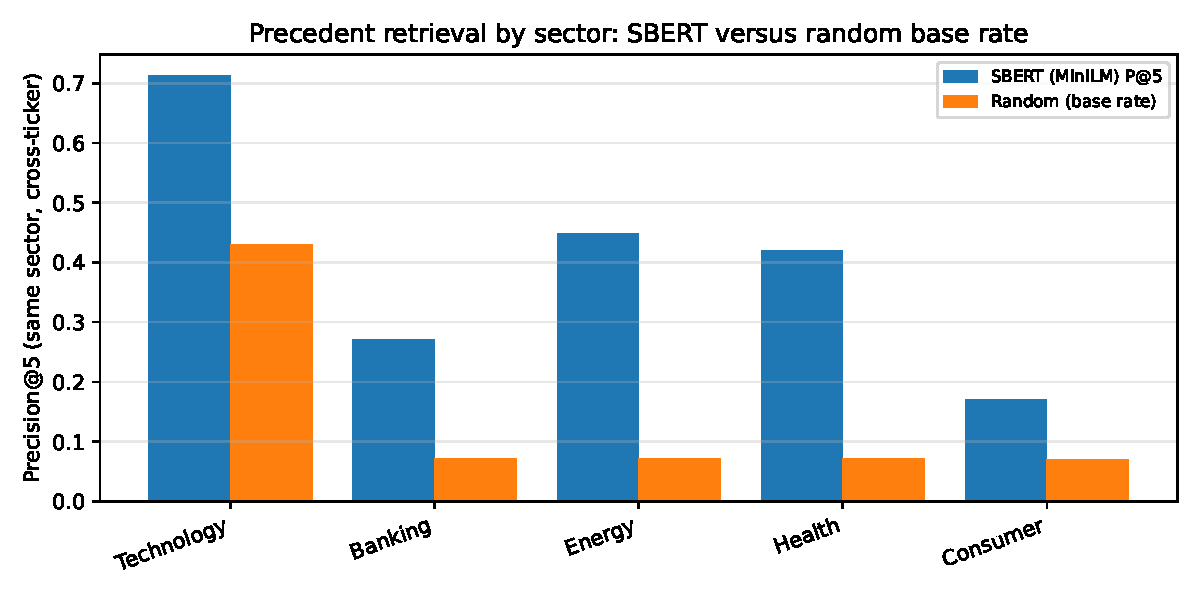
\includegraphics[width=\linewidth]{eval_retrieval_per_sector.pdf}
\par\scriptsize Ganho maior onde o vocabulário é distintivo (energia, saúde).
\end{columns}
\vspace{1mm}\par\centering\footnotesize Validado à escala no FNSPID multi-ano (${\sim}80$k manchetes): \textbf{P@5 $0.595$}; consistência de direção $0.71$ no chão do acaso $0.69$ (tema, não direção).
\end{frame}

\begin{frame}{Resultado 3: as explicações são fiéis por construção}
\begin{columns}
\column{0.52\textwidth}
\begin{itemize}\small
  \item Cada alerta é composto \emph{diretamente} a partir dos objetos calculados.
  \item Por isso o texto \textbf{não pode divergir} do cálculo.
  \item Verificado por um teste automático (o alerta reproduz a data/ticker/impacto de cada precedente).
  \item Cada alerta termina com um aviso de não-previsão.
\end{itemize}
\column{0.48\textwidth}
\begin{block}{\scriptsize Alerta real (gatilho de notícias)}
\tiny\ttfamily
News alert --- NVDA\\
``Nvidia raises guidance\ldots AI data-centre''\\
Avg 1-day move: $-1.97\%$ (over 5; 3 shown)\\
- MSFT (0.68) +1d $-3.46\%$\\
- META (0.68) +1d $-2.65\%$\\
- GOOGL (0.64) +1d $-0.46\%$\\
\emph{observed past outcome, not a prediction}
\end{block}
\end{columns}
\end{frame}

\begin{frame}{Resultado 3b: a mesma garantia, para linguagem gerada}
\begin{columns}
\column{0.52\textwidth}
\small
Um modelo de linguagem foi acrescentado \textbf{estritamente como narrador}: pode redigir a
evidência, nunca fornecê-la. Uma guarda valida cada resposta antes da entrega e
\textbf{descarta-a inteira} perante:
\begin{itemize}\small
  \item um número ausente da evidência,
  \item um valor com o \textbf{sinal} invertido,
  \item formulação preditiva ou de conselho,
  \item uma atribuição que contradiga a calculada.
\end{itemize}
A garantia é propriedade \textbf{do sistema}, não do modelo portar-se bem.
\column{0.48\textwidth}
\begin{block}{Dois números, de propósito}
\small
\textbf{Pré-guarda:} o modelo cru violou a evidência em alguns casos.\\
\emph{$\Rightarrow$ é por isto que a guarda existe.}\\[4pt]
\textbf{Entregue:} \textbf{zero} violações.\\
\emph{$\Rightarrow$ é a guarda que está em julgamento.}
\end{block}
{\footnotesize\textbf{Ressalva honesta:} o segundo é em parte circular, já que o mesmo
verificador decide e avalia. O contrapeso é um corpus de red team: um exercício independente
partiu o \emph{primeiro} desenho (uma blocklist) com 29 contornos reproduzidos. O espaço de
paráfrases é ilimitado e qualquer lista dele é finita, por isso a guarda foi reconstruída como
\textbf{vocabulário fechado}. Esses ataques são hoje testes de regressão permanentes.}
\end{columns}
\end{frame}

\begin{frame}{Resultado 4: triagem aprendida --- treinada, calibrada, honesta}
\begin{columns}
\column{0.55\textwidth}
\begin{itemize}\small
  \item \textbf{Tarefa:} $P(\text{movimento anormal segue a notícia})$ --- materialidade, \textbf{nunca} direção. Rótulos do nosso próprio estudo de evento ($|$ticker $-$ SPY$| \ge 2\%$ em $(d,d{+}3]$).
  \item \textbf{Corpus:} FNSPID 2018--2023, $79{,}753$ exemplos; split temporal por dia + embargo; calibração só na validação.
  \item \textbf{Anti-lookahead:} um teste unitário \emph{muta os preços futuros} --- features inalteradas, rótulo muda.
\end{itemize}
\column{0.45\textwidth}
\scriptsize
\begin{tabular}{l c c}
\toprule
Modelo & PR-AUC & P@5/dia \\
\midrule
Sempre (base) & 0.378 & 0.163 \\
\textbf{Volatilidade LR} & \textbf{0.542} & \textbf{0.632} \\
Contexto LR & 0.538 & 0.632 \\
Contexto$+$texto LR & 0.496 & 0.585 \\
Gradient boosting & 0.469 & 0.551 \\
\bottomrule
\end{tabular}
\end{columns}
\vfill
\begin{block}{\small O veredicto honesto (pré-comprometido)}
\small Dentro de um orçamento de 5 alertas/dia, a triagem quase \textbf{quadruplica a precisão} ($0.632$ vs $0.163$) --- mas \textbf{nenhum modelo de texto bateu a volatilidade}. Uma ablação de seguimento juntou \emph{cinco} features de contexto baratas (regime de mercado, momentum, reação padronizada, risco de queda): PR-AUC $0.535$, de novo \textbf{sem ganho}. Um re-teste \emph{justo} (C afinado, texto reduzido por PCA, um encoder de domínio FinBERT) continua a não bater a volatilidade, pelo que o negativo é \textbf{robusto}, não um artefacto de sub-ajuste. O sinal é o contexto de mercado; reportado tal como se revelou.
\end{block}
\end{frame}

\begin{frame}{O produto, ao vivo}
\begin{columns}
\column{0.55\textwidth}

\includegraphics[width=\linewidth]{app_dashboard.png}
\column{0.45\textwidth}
\small
Uma captura genuína, não um mockup. \textbf{Três ecrãs, um por pergunta:}
\begin{itemize}\small
  \item \textbf{Today} --- a watchlist ordenada por quão longe do normal, com a repartição
        mercado/setor/empresa \textbf{na própria linha}. Sem clicar.
  \item \textbf{Ticker} --- gráfico, decomposição por extenso, e os alertas \emph{exatamente}
        como o canal Telegram os recebeu. Nunca recalculados.
  \item \textbf{Method} --- os números congelados, incluindo o resultado negativo.
\end{itemize}
{\footnotesize A promessa aparece \textbf{uma} vez, como identidade da página. O valor de
latência é \textbf{medido} e está simplesmente ausente quando os carimbos não existem.}
\end{columns}
\end{frame}

\newcommand{\techbadge}[2]{{\setlength{\fboxsep}{3pt}\colorbox{#1!13}{\small\strut #2}}}
\newcommand{\techcat}[1]{\smallskip\par\textbf{\footnotesize #1}\par\smallskip}
% Logo real se slides/logos/<file>.png existir; senao um badge de nome limpo (ver logos/README.md).
\newcommand{\techlogo}[3]{\IfFileExists{logos/#1.png}%
  {\raisebox{-3pt}{\includegraphics[height=13pt]{logos/#1.png}}~}{}\techbadge{#2}{#3}}
\begin{frame}{Feito com --- ferramentas gratuitas e dados abertos, de ponta a ponta}
\centering\vspace{1mm}
\techcat{\textcolor{blue!60}{Fontes de dados \& APIs}}
\techlogo{huggingface}{blue}{FNSPID (Hugging Face)}\ \techlogo{yfinance}{blue}{yfinance}\ %
\techlogo{finnhub}{blue}{Finnhub}\ \techlogo{rss}{blue}{feeds RSS}\ \techbadge{blue}{SPY (proxy de mercado)}
\techcat{\textcolor{orange!75!black}{Aprendizagem automática}}
\techlogo{sbert}{orange}{Sentence-BERT / MiniLM}\ \techlogo{scikit-learn}{orange}{scikit-learn}\ %
\techlogo{pytorch}{orange}{PyTorch (CPU)}\ \techbadge{orange}{calibração de Platt}\ %
\techlogo{onnx}{orange}{ONNX Runtime}
\techcat{\textcolor{green!55!black}{Produto \& entrega}}
\techlogo{telegram}{green}{Telegram Bot API}\ \techlogo{streamlit}{green}{Streamlit}\ %
\techlogo{plotly}{green}{Plotly}
\techcat{\textcolor{purple!70}{Engenharia \& infraestrutura}}
\techlogo{python}{purple}{Python 3.12}\ \techlogo{githubactions}{purple}{GitHub Actions (cron)}\ %
\techlogo{pytest}{purple}{pytest $+$ ruff}\ \techbadge{purple}{joblib}
\par\bigskip
{\footnotesize Sem APIs pagas, sem GPUs, sem servidor sempre ligado --- reprodutível num portátil.}
\end{frame}

\begin{frame}{Limitações (enunciadas com clareza)}
\begin{itemize}
  \item A relevância é um \textbf{indicador aproximado por mesmo setor}, não um juízo humano.
  \item O corpus de recuperação é uma janela \textbf{recente} da camada gratuita (entretanto validada à escala no FNSPID, P@5 $0.595$); o estudo de \emph{triagem} usou de facto o FNSPID multi-ano (14/15 tickers --- a Meta é ``FB'' no corpus).
  \item O impacto de precedente mostrado é um retorno pós-evento \textbf{bruto} (os rótulos de triagem \emph{são} ajustados ao mercado).
  \item A similaridade é \textbf{temática, não direcional}: um agrupamento pode misturar movimentos de subida/descida, pelo que a média é \emph{evidência} ao nível do tema, não uma previsão.
  \item \textbf{Ainda sem estudo humano de utilidade} (utilidade da RQ3 em aberto).
  \item Por desenho: \textbf{sem previsão de preços, sem negociação}, pelo que as métricas de lucro estão fora de âmbito.
\end{itemize}
\vfill
\footnotesize Todos os resultados são reprodutíveis a partir de scripts versionados (re-correr: números idênticos).
\end{frame}

\begin{frame}{Conclusões}
\begin{itemize}
  \item \textbf{RQ1 (sim):} o \emph{z}-score transparente deteta de forma consistente em todo o mercado e explica cada marca.
  \item \textbf{RQ2 (sim, validada à escala):} a recuperação semântica muito acima das linhas de base (P@5 $0.595$ no FNSPID multi-ano); impacto medido sem lookahead.
  \item \textbf{RQ3 (fiel sim; útil em aberto):} as explicações não podem divergir do cálculo; a utilidade para humanos é trabalho futuro.
  \item \textbf{RQ4 (não no texto; sim no mecanismo):} a triagem $\approx 4\times$ de precisão dentro do orçamento, mas a volatilidade ficou imbatida --- o \emph{segundo} teste justo ``aprendido vs simples'' que a escolha transparente venceu (o primeiro: Isolation Forest vs \emph{z}-score, $F_1$ $0.271$ vs $0.530$).
\end{itemize}
\vfill
\begin{block}{Contribuição}
Um sistema de alertas financeiros funcional, \textbf{explicável e reprodutível} para investidores de retalho --- componentes existentes mais um modelo de triagem treinado pelo autor, engendrados num todo transparente, com uma avaliação honesta.
\end{block}
\end{frame}

\begin{frame}{Obrigado}
\vfill
\centering
{\Huge \textbf{InvestiGator}} \\[4mm]
{\large Alertas financeiros explicáveis para investidores de retalho} \\[8mm]
{\footnotesize Perguntas são bem-vindas.}
\vfill
\end{frame}

\begin{frame}{Perguntas antecipadas}
\footnotesize
\begin{itemize}
  \item \textbf{Porquê não prever preços?} Eficiência de mercado (Fama 1970): as notícias públicas são absorvidas depressa; nós \emph{medimos} reações, honestamente.
  \item \textbf{Porquê \emph{z}-score, não Isolation Forest/GARCH?} Transparência para um sinal de baixa dimensão --- e \emph{testámo-lo}: uma Isolation Forest causal sobre a mesma informação perdeu ($F_1$ $0.271$ vs $0.530$).
  \item \textbf{O vosso modelo treinado perdeu para a linha de base da volatilidade. Fracasso?} Não: a comparação foi \emph{pré-comprometida} e responde à RQ4 com evidência; a triagem ainda dá $\approx 4\times$ de precisão dentro do orçamento vs alertar sempre, e a variante em produção usa exatamente as features que carregam o sinal.
  \item \textbf{Como sabem que o modelo de triagem nunca vê o futuro?} Um teste unitário muta os preços pós-evento e verifica que as features ficam inalteradas enquanto o rótulo muda; split temporal por dia único com um embargo de cinco dias.
  \item \textbf{Porquê precisão@$k$ e um proxy de setor?} Métrica padrão de recuperação ordenada; objetiva, reprodutível; a relevância humana é trabalho futuro.
  \item \textbf{Restrição cross-ticker?} Uma escolha de \emph{avaliação} para evitar auto-correspondências triviais; o alerta ao vivo mostra os precedentes mais similares, seja qual for a empresa.
  \item \textbf{Uma manchete positiva recuperou precedentes negativos ($-1.97\%$). Enganador?} A similaridade capta o \emph{tema}, não a direção; a média é \textbf{evidência} ao nível do tema, mostrada com cada precedente e um aviso de não-previsão. Trabalho futuro: de-duplicar precedentes e sinalizar divergência de direção.
  \item \textbf{É reprodutível?} Sim: sementes fixas, dependências fixadas, scripts versionados; re-correr reproduz cada número.
\end{itemize}
\end{frame}

\begin{frame}{Perguntas antecipadas (continuação)}
\footnotesize
\begin{itemize}
  \item \textbf{``Zero violações entregues'' não é circular, se é o vosso próprio verificador
        a avaliar?} Em parte é, e a tese di-lo. Por isso não é o único teste: um red team
        independente partiu a guarda \emph{anterior} com 29 contornos reproduzidos, construídos
        sem ver o desenho atual, e esses ataques são hoje testes de regressão.
  \item \textbf{Então construíram um sistema multi-agente?} Não, e não o vou reivindicar. Um
        modelo a chamar algumas funções não é multi-agente. O narrador é uma \textbf{função
        pura} da evidência para um parágrafo.
  \item \textbf{Porquê excluir os price targets de analistas? São gratuitos.} Porque importar a
        previsão de outra pessoa para um sistema definido por não prever é uma contradição.
        Preferiu-se a coerência à cobertura, e está enunciado como posição no Capítulo~6.
  \item \textbf{Porquê nenhuma funcionalidade de carteira?} As posições são dados financeiros
        pessoais, e ``as tuas maiores posições são uma só aposta'' é aconselhamento, seja qual
        for a redação. Isso atravessa a fronteira de que a afirmação ética depende.
  \item \textbf{De onde vem o limiar de triagem $0{,}5$?} Originalmente de lado nenhum, que era
        o problema honesto. Varrê-lo sob um rácio de custo explícito mostrou que assumia
        implicitamente que uma falha custa aproximadamente o mesmo que um falso alarme; sob
        custos iguais o ótimo fica onde a constante já estava. Vindicado, mas agora \emph{derivado}.
  \item \textbf{Os vossos alertas chegam horas atrasados.} Medido: mediana de cerca de três
        horas, e a causa é o agendador gratuito, não o método. O caminho sempre-ligado está
        escrito e custa cerca de um minuto; implantá-lo ficou fora do âmbito da avaliação, e o
        número honesto está \textbf{à vista no produto} em vez de escondido.
\end{itemize}
\end{frame}

\end{document}
